%----------------------------------------------------------------------------------------
%	Using Mathematica for Data Analysis
%----------------------------------------------------------------------------------------

\chapterimage{chapter_head_1.pdf} % Chapter heading image

\chapter{Using Mathematica for Data Analysis}

Besides being a great program for doing complicated algebraic calculations and working the calculus we're too lazy or pressed for time to slog through, Mathematica is a great program for basic plotting and fitting, and has many built in features which can instantly render figures and tables for use in a paper or lab report.


\section{Running commands}
\begin{remark}
If you've never used Mathematica ever before in your life, it may be useful to read this section.
\end{remark}
Mathematica is structured so as to act like a notebook you write down your equations in and manipulate your theoretical ideas. To make the feel of this program work, the software does not run like an ordinary scripting language. Instead of writing a program and executing a file, Mathematica evaluates one line at a time. This has some advantages, as you can change everything on the fly, but it may be confusing at first if you've never seen it before or are expecting to ``compile'' the whole program.

\subsection{Conventions}
 When entering commands in Mathematica, a few command conventions hold:
\begin{enumerate}
\item Commands always begin with capital letters and use square brackets (\texttt{[]}) are used for command arguments or as locations in a matrix when used twice ( e.g \texttt{[[]]})
\begin{example} Function arguments: \texttt{ListPlot[]}, \texttt{Table[]} \end{example}
\begin{example} Location in a matrix or ``table":  \texttt{A[[1,2]]} refers to the element in the first row and second column of matrix \texttt{A} \end{example}
\item Parentheses are used to group terms in an equation or an expression and are \emph{not} used in functions or denoting function arguments at all.
\item Greek letters like $\alpha$, $\beta$, $\gamma$ etc. are obtained by sandwiching the corresponding roman letters between escape characters. For instance, press escape then the letter \texttt{a} followed by escape again -- you should get $\alpha$. 
\end{enumerate}


\section{Loading data}
\begin{sloppypar}
Two common ways to import data are the \texttt{Import["file.txt","Format"]} and the \texttt{ReadList["file.txt","Format"]} functions.  On the computers in the PMCL, Mathematica will look specifically in your Documents folder for the data file you specify. One way to check whether this is true (it {\it might not be}) is to execute  the command \texttt{Directory[]}: this command will tell you where Mathematica is looking for files. However, if you give Mathematica the full file path, it will know exactly where to go.
\end{sloppypar}
Once your data files are in this folder (e.g. \texttt{"C:\textbackslash Users\textbackslash}$uteid$\texttt{\textbackslash Documents"}), you can simply use \texttt{Import[]} and \texttt{ReadList[]} without providing the full file address. This is a fast way to work if you like to download your files off of your email and continually send the updated versions to yourself. If you have a flashdrive however, a much more efficient solution can be found in useful tip \ref{UTuploadingdata}

\begin{example}
\texttt{rawdata = Import["Filewithdata.txt", "Table"];}
\end{example}
\begin{example}
\texttt{rawdata = ReadList["Filewithdata.txt", Number, RecordLists}$\to$\texttt{True];}
\end{example}

\begin{exercise}[Probably the most convenient solution to uploading data]


If you would like to change directories, for instance if you like to work off of a flash drive, you can quickly access files that are in the same folder as your notebook by using the \texttt{NotebookDirectory[]} command. The way to do this is by {\it concatenating} the notebook directory with the file name you're interested by using the \texttt{<>} between \texttt{NotebookDirectory[]} and \texttt{"Filewithdata.txt"}. The string you give Mathematica is then a complete filepath description of where the file is, and so this is very robust and useful. For example:

\begin{example}
If you have both your data file and your notebook file in a folder on a flash drive, let's call it \texttt{Flashdrive Folder}, and you want to import a text file with only comma-separated or tab-delimited data, you can use the following command and obtain a matrix with all of the data:\\\\
\texttt{rawdata = Import[NotebookDirectory[] <> "Sample0001.txt", "Table"];}\\ \\
Here, \texttt{NotebookDirectory[] <> "Sample0001.txt"} retrieves the string for the filepath \\ \texttt{I:\textbackslash Flashdrive Folder\textbackslash Sample0001.txt}. {\bf This means that every time you move \texttt{Flashdrive Folder}, Mathematica will be able to find the data files and you won't have any problems.}

If the file contains non-number (strings) in any of the columns, it is more useful to use the \texttt{Readlist[]} command as you can specify which columns don't contain numerical data. Let's say you have three columns in your \texttt{.txt} file where your first column specifies the date and the second and third  contain numerical data. By putting the list \texttt{\{Word, Number, Number\}} in as an option, Mathematica knows that the data in the first column are words and not numbers: \\
\\
\texttt{rawdata = }\\\texttt{  ReadList[NotebookDirectory[] <> "Sample0001.txt", \{Word, Number, Number\}]};\\
\\
In general, if you just want to input a datafile with only a matrix matrix, use:\\
\\
\texttt{rawdata =} \\ \texttt{ ReadList[NotebookDirectory[]<>"Sample0001.txt",  Number, }\texttt{RecordLists}$\to$\texttt{True];}
\end{example}
\label{UTuploadingdata}
\end{exercise}
%------------------------------------------------

\section{Plotting numerical data}\index{Figure}

To plot two columns of numerical data against eachother in Mathematica, you can't just give Mathematica two lists of data to plot. This is because the program likes to think of plotting numbers in terms of $\{x,y\}$ pairs. Instead, if you have a matrix ( \texttt{data}) with columns of numerical values imported correctly, you will have to construct a list of pairs. Once you get the hang of this, it can become reasonably intuitive. If you're used to Excel or MATLAB, it might be confusing at first though.

\begin{example}\index{Plotting in Mathematica}
To plot data in column 1  against data in column 2 of an imported dataset \texttt{data}, use: \texttt{ListPlot[data[[All,\{1,2\}]], AxesLabel }$\to$ \texttt{\{"Column 1", "Column 2"\},}\\ \texttt{
 ImageSize $\to$ Large]}\\

\end{example}
At the end of the command, \texttt{AxesLabel} and \texttt{ImageSize} are {\it options} that Mathematica has built-in settings for. If you are ever confused about what these options do, search the documentation for the function you're using and click on ``details'' on that page. This should tell you everything you need to know about what the function can do.  


\begin{figure}[h]
\centering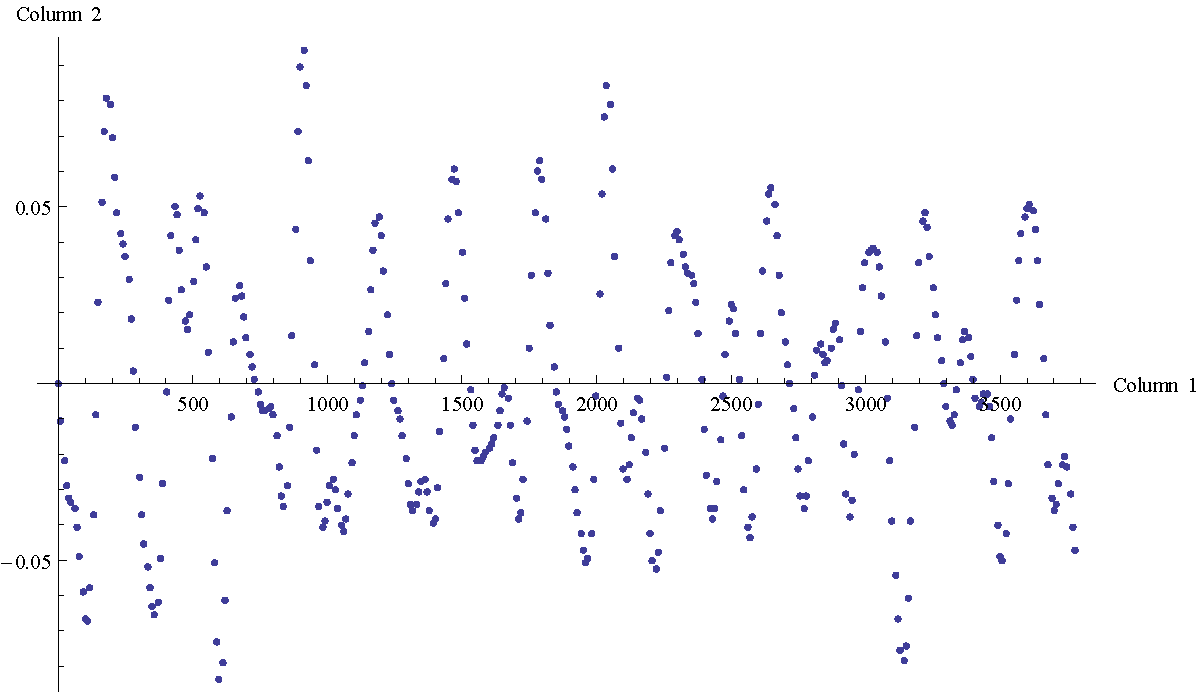
\includegraphics[scale=0.7]{listplot.pdf}
\caption{A \texttt{ListPlot[]} of sample data. One thing you may notice about this  plot is that it is rather cluttered and doesn't convey the fact that it is a timeseries very well. Also, the axes font isn't very readable at this scale.}
\end{figure}
To make the plot more readable, there are many options one can use in \texttt{ListPlot[]} or \texttt{ListLinePlot[]}. Some common options include:
\begin{enumerate}
\item {\bf Making axes font bigger:} \texttt{BaseStyle $\to$ \{FontSize $\to$ 20\}}, or whatever pt font you would like to use. The \texttt{BaseStyle} option includes ways of making the fonts bold or italic as well.
\item {\bf Titling plots:} \texttt{PlotLabel $\to$ "Title"} \texttt{PlotLabel $\to$ Style["Title", "Style"]}. Mathematica has a lot of style formats like `` Graphics'' and ``Section'' which mimic Mathematica's typsetting features. These can look pretty good at times, but it's a good habit to use \LaTeX $\;$ for plot titles if you can get that to work.
\item {\bf Adding grid lines:} \texttt{GridLines $\to$ Automatic}. This puts grid lines on the plot in a basic unassuming way. To make the lines dashed use \texttt{GridLineStyle $\to$ Dashed}. You can also specify where the grid lines are and change the color.

\end{enumerate}

\begin{figure}[h]
\centering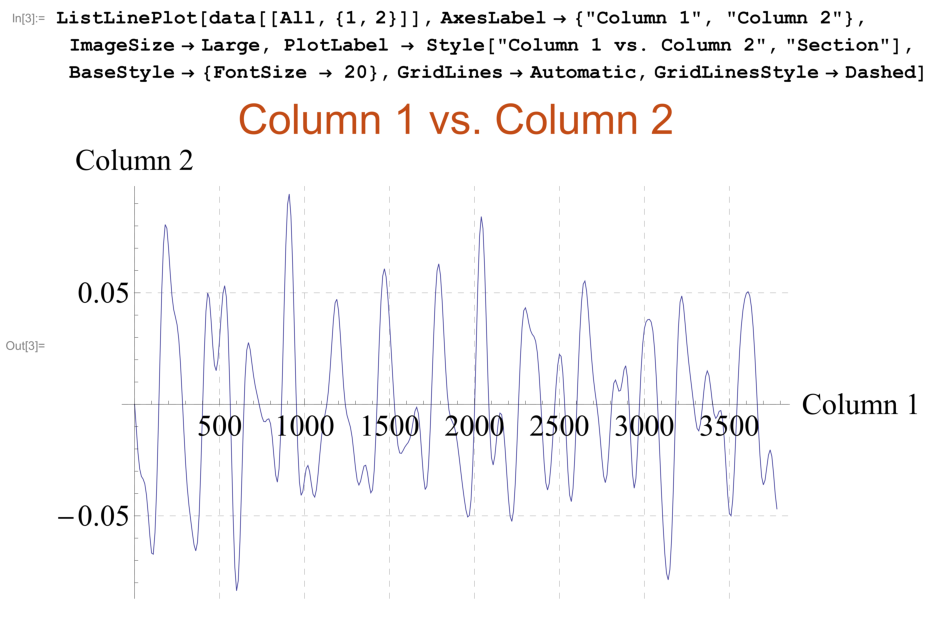
\includegraphics[scale=1]{complexplottingexample.pdf}
\caption{As you can see, this plot is more easy to look at and showcases the basic plotting options.}
\label{fig:listlineplot}
\end{figure}
\subsection{Histograms}
Making histograms is very straightforward using the \texttt{Histogram[$list$, $bins$]} command
\begin{figure}[H]
\centering 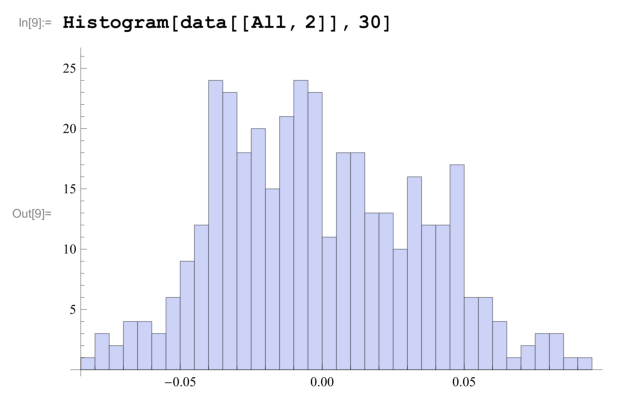
\includegraphics[scale=1]{histogramexample.pdf}
\caption{A histogram of a column of data}
\label{fig:histexample}
\end{figure}


\newpage
\section{Tables and Grids}
In mathematica, it is fairly straightforward to make a table of data with formatted headers. What mathematica needs to see is a matrix or list-of-lists of some form that can be put into a grid. In the example below, the code creates a column of means and a column of standard deviations for 18 columns of data, and then puts this information into a table with labelled columns and rows using the \texttt{TableForm[]} command:
\begin{figure}[H]
\centering 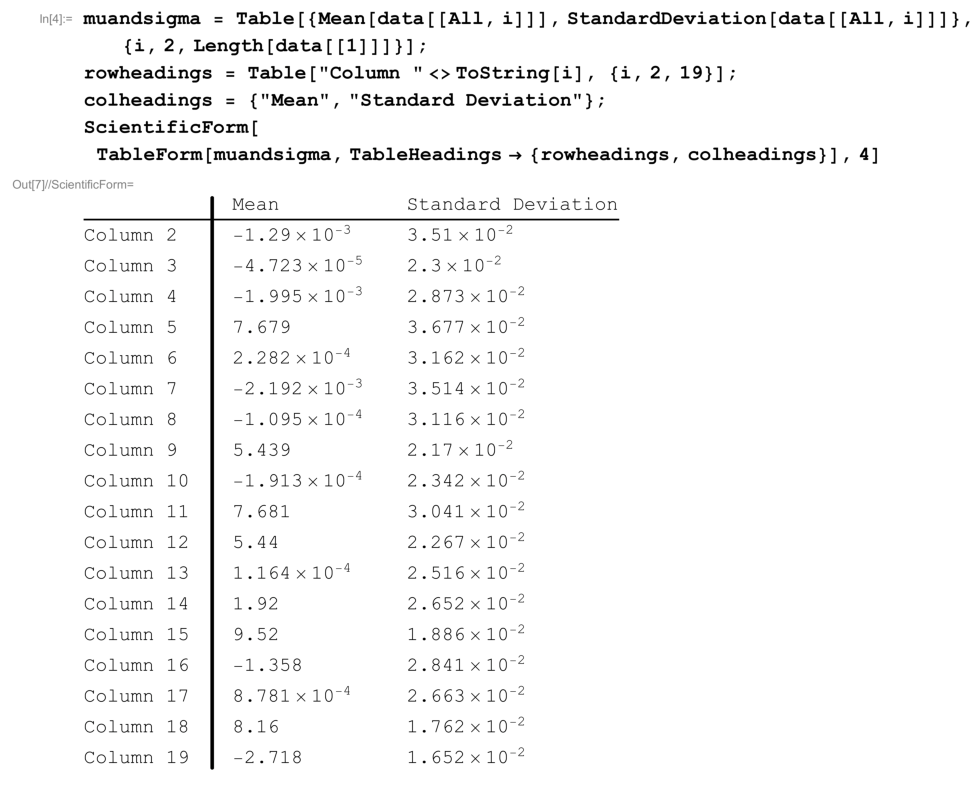
\includegraphics[scale=.97]{tableexample.pdf}
\end{figure}
\newpage
\section{Fitting arbitrary functions to data}
If you have some data and you are interested in fitting it with some nonlinear function, mathematica can do that without having to install a toolbox like MATLAB requires. The way to do this is to take some data and use the \texttt{NonlinearModelFit[]} command. In the example below, the data used in figure \ref{fig:histexample} is fit with a gaussian function. Because mathematica outputs a set of histogram bin edge positions instead of bin centers, the first four lines of the example are used to prepare a dataset that can be fit with a gaussian.
\begin{figure}[H]
\centering 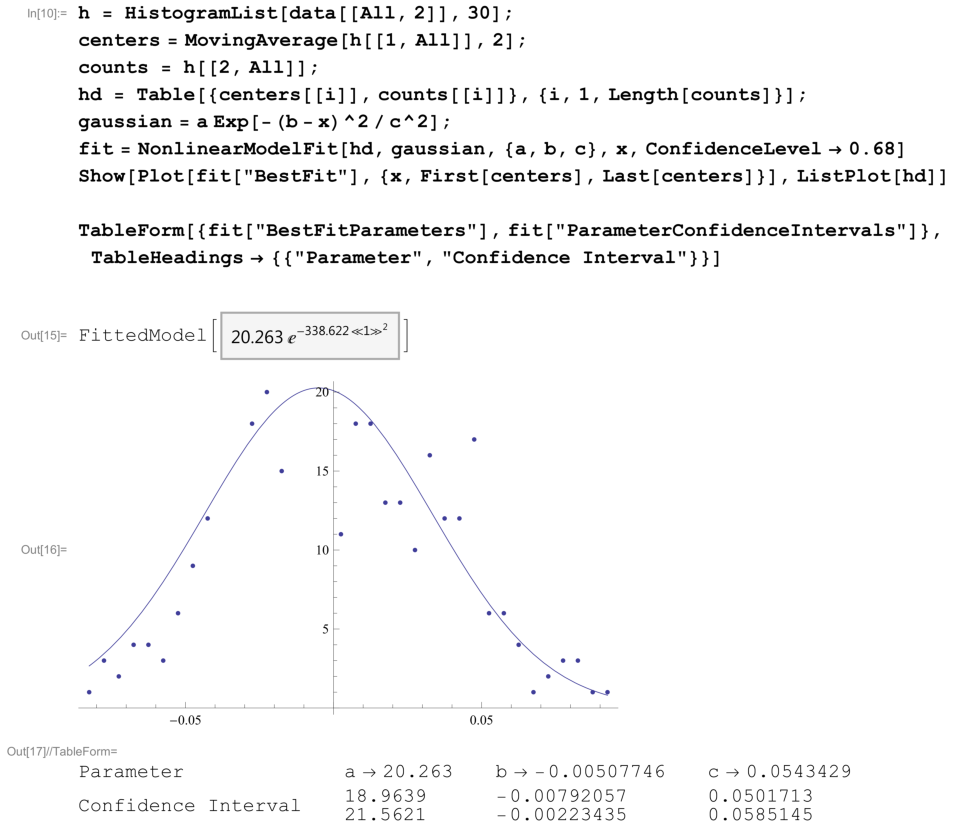
\includegraphics[scale=1]{basicfittingexample.pdf}
\end{figure}
This example again makes use of the \texttt{TableForm[]} command, useful for bundling the parameters and confidence interval informations into a table for easy reading. The general idea here is that \texttt{NonlinearModelFit[]} returns (creates) an object we decided to call \texttt{fit}.

\begin{exercise}[Interpretting this data: why \texttt{ConfidenceLevel} is important]
The parameters and confidence intervals of this model have been estimated using a nonlinear least-squares algorithm. This means that the uncertainties in the parameters have already been found, assuming that the noise in the data is uniformly distributed. So, if we want to read off uncertainties in the standard format of $\hat x \pm \hat \sigma_x$, all we need to do to find $\hat \sigma_x$ is divide the width of the confidence interval by two (the confidence interval takes up 2$\hat\sigma$). If \texttt{ConfidenceLevel$\to$ 0.95}, then the confidence interval would take up about 4$\hat \sigma$ instead. This comes from the standard normal distribution.
\end{exercise}